\clearpage{}
\section{Cite and briefly describe, with small examples, the types of
notation that can be used to describe the structure, the behaviour or the
functions of a system. Define and distinguish the notions of verification
and validation, and the techniques that can apply to them. Explain how
they apply to requirements.}

\subsection{Types of notation to describe the structure, the behaviour or the functions
of a system}

\subsubsection{Structure}

\begin{itemize}
    \item Entity-Relationship diagram (ER diagram)
    \item Class diagram
\end{itemize}

\subsubsection{Behaviour}

\begin{itemize}
    \item Event traces
    \item Sequence diagram
    \item State diagram
    \item Petri nets
    \item Data-flow diagram
    \item Use-case diagram
\end{itemize}

\subsubsection{Functions}

\begin{itemize}
    \item Decision table
    \item Parnas table
    \item Object constraint language (OCL)
    \item Algebraic specifications
\end{itemize}

\subsection{Notions of verification and validation}

\begin{description}
    \item[Verification] Specifications conform to requirements (i.e. \enquote{build the right system})
        \subitem{} $\rightarrow$ documents $\div$ documents (easier)
    \item[Validation] Requirements accurately reflects the customer's needs (i.e. \enquote{build the system right})
        \subitem{} $\rightarrow$ needs $\div$ documents (harder)
\end{description}

\begin{figure}[!ht]
    \centering
    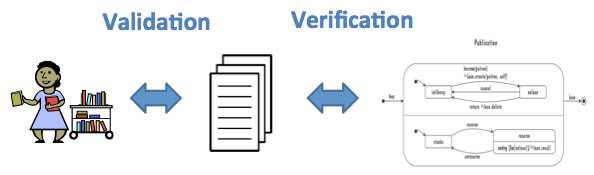
\includegraphics[width=0.7\linewidth]{validation_verification.png}
    \caption{Validation and verification}
\end{figure}

\subsubsection{Techniques that apply to them}

\begin{table}[!ht]
    \begin{center}
        \begin{tabular}{cc}
            \toprule
            Verification            & Validation \\
            \midrule
            Cross-referencing       & Walkthrough \\
            Simulation              & Readings \\
            Consistency checks      & Interviews \\
            Completeness checks     & Reviews \\
            Reachability checks (states, transitions) & Checklists \\
            Model checking          & Formal inspections \\
            Mathematical proofs     & Modeling \\
                                    & Scenarios \\
                                    & Prototypes \\
                                    & Simulation \\
            \bottomrule
        \end{tabular}
    \end{center}
\end{table}

\subsubsection{How they apply to requirements}

\paragraph{Verification}

Check that specifications are conforming to definitions and to other specifications (consistency). \newline
Check traceability or (better) demonstrate.
\begin{center}
Specification \textbf{and} assumptions \textbf{imply} requirements
\end{center}
Eventually computer helped (model checking or theorem proving).

\paragraph{Validation}

Review of the requirements by representatives of the customer and the developer. Meeting to discuss the result. \newline

Steps:

\begin{itemize}
    \item Review the goals and objectives of the system
    \item Compare requirement with goal and objectives
    \item Review environment in which the system operates
    \item Etc\ldots
\end{itemize}
